
\section{Allgemein}
	\subsection{Schaltelemente bei zeitabhängigen Vorgängen}
	\begin{tabular}{p{1.5cm} p{4.3cm} p{1.5cm} p{4.3cm} p{1.5cm} p{4.3cm}}
   		\multicolumn{2}{l}{\textbf{Ohmscher Widerstand R}}
   			& \multicolumn{2}{l}{\textbf{Kapazitität C}}
   			& \multicolumn{2}{l}{\textbf{Induktivität L}} \\
   		\multicolumn{2}{l}{$u$ und $i$ können sprunghaft ändern}
   			& \multicolumn{2}{l}{$u$ kann nicht sprunghaft ändern}
   			& \multicolumn{2}{l}{$i$ kann nicht sprunghaft ändern} \\
   		\parbox{1.5cm}{
			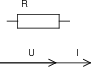
\includegraphics[width=1.5cm]{./bilder/zeigerdiag-r.png}}
			& \parbox{4.3cm}{$u(t) = R i(t)$ \\
				$i(t) = \frac{u(t)}{R}$ \\
				$\underline{Z} = R$}
   			& \parbox{1.5cm}{
				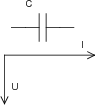
\includegraphics[width=1.5cm]{./bilder/zeigerdiag-c.png}}
			& \parbox{4.3cm}{
				$u(t) = \frac1C \int\limits_0^t i(\tau) d\tau + u(0)$ \\
				$i(t) = C \frac{d u(t)}{dt}$ \\
				$\underline{Z} = \frac{1}{j \omega C} = - \frac{j}{\omega C}$ \\
				$W_C=\frac12 C U_C^2$}
   			& \parbox{1.5cm}{
				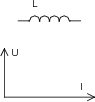
\includegraphics[width=1.5cm]{./bilder/zeigerdiag-l.png}}
			& \parbox{4.3cm}{
				$u(t) = L \frac{di(t)}{dt}$ \\
				$i(t) = \frac1L \int\limits_0^t u(\tau) d\tau + i(0)$ \\
				$\underline{Z} = j \omega L$ \\
				$W_L=\frac12 L I_L^2$}
   	\end{tabular}

	\subsection{Vorgehen bei Schaltvorgängen}
		\fbox{$u(t) =U_E + (U_A - U_E) e^{\frac{-t}{\tau}} \qquad \tau = C R \text{ bzw. }
		\tau =
		 \frac{L}{R} = \frac{\varepsilon}{\sigma} \qquad U_A = \lim\limits_{t
		 \rightarrow 0^+} u(t) \qquad U_E =
		 \lim\limits_{t \rightarrow \infty} u(t)$} $\qquad$ Für Ströme äquivalent
		 
		 \subsection{Taschenrechner TI-89/Voyage 200 englisch}
		 	\begin{tabular}{p{6cm} p{12cm}}
				 \texttt{comDenom(Z/N, x)} & Gemeinsamen Nenner finden \\
				 \texttt{cZeros($\ldots p^m \ldots$ | p = i * $\omega$, $\omega$)} &
				 Komplexe Nullstellen finden (für Pole jeweils Nenner der UTF einsetzen) \\
				 \texttt{expand($p^n/q^m$)} & Partialbruchzerlegung \\
				 \texttt{propFrac($p^n/q^m$)} & Polynomdivision \\
				 \texttt{pds$\backslash$partial($\{a_n, \ldots, a_0\},\{b_m, \ldots, b_0\}$)} & 100\%-ige
				 Partialbruchzerlegung, \textcolor{red}{Root-Folder}: Mode
				 $\rightarrow$ Current Folder $\rightarrow$ pds \\ 
				 \texttt{pds$\backslash$roots($\{a_n, \ldots, a_0\}$)} & Nullstellen
				 bestimmen \\ \texttt{acst$\backslash$laplace($f(t)$)} & Laplacetransformation \\
				 \texttt{acst$\backslash$invlap($F(s)$)} & inverse Laplacetransformation   
			\end{tabular}
		 
		 
	\subsection{Vektor -/ Kreuzprodukt, Rechte-Hand-Regel}
	$\vec{c} = \vec{a} \times \vec{b}$: \qquad $\vec{a} \Leftrightarrow$ Daumen;
	$\vec{b} \Leftrightarrow$ Zeigefinger; $\vec{c} \Leftrightarrow$ Mittelfinger
	 
	 \subsection{Partialbruchzerlegung\formelbuch{15}}
		Falls möglich, erst Polynomdivision.
		\[f(x)=\frac{x^2+20x+149}{x^3+4x^2-11x-30} \Rightarrow \; \begin{array}{l}\text{Nenner faktorisieren mit}\\
		\text{Hornerschema\formelbuch{914}, Binom, etc.}\end{array} \Rightarrow x^{3}+4x^{2}-11x-30=(x+2)(x^{2}+2x-15)=(8x+2)(x+5)(x-3)\]
		Ansatz:
		\[f(x)=\frac{x^2+20x+149}{x^3+4x^2-11x-30}=\frac{A}{x-3} + \frac{B}{x+2} + \frac{C}{x+5}=
		\frac{A(x+2)(x+5)+B(x-3)(x+5)+C(x-3)(x+2)}{(x-3)(x+2)(x+5)}\]
		Gleichungssystem aufstellen mit beliebigen $x_i$-Werten (am Besten Polstellen oder 0,1,-1 wählen):
		\[\begin{array}{l}x_1=3:\;-9+60+149=A\cdot5\cdot8\;\;\;\Rightarrow A=5\\
		x_2=-2:\;-4-40+149=B(-5)\cdot3\; \Rightarrow B=-7\\
		x_3=-5:\;-25-100+149=C(-8)(-3) \Rightarrow C=1 \end{array} \Rightarrow f(x)=\frac{5}{x-3}+\frac{7}{x+2}\frac{1}{x+5}\]
		weitere Ansätze für andere Typen von Termen:
		\[f(x)=\frac{5x^2-37x+54}{x^3-6x^2+9x}=\frac{A}{x}+\frac{B_1}{x-3}+\frac{B_2}{(x-3)^2}=\frac{A(x-3)^2+B_1x(x-3)+B_2x}{x(x-3)^2}\]
		\[f(x)=\frac{1,5x}{x^3-6x^2+12x-8}=\frac{A_1}{x-2}+\frac{A_2}{(x-2)^2}+\frac{A_3}{(x-2)^3}=\frac{A_1(x-2)^2+A_2(x-2)+A_3}{(x-2)^3}\]
		\[f(x)=\frac{x^2-1}{x^3+2x^2-2x-12}=\frac{A}{x-2}+\frac{Bx+C}{x^2+4x+6}=\frac{A(x^2+4x+6)+(Bx+C)(x-2)}{(x-2)(x^2+4x+6)}\]
	\subsection {Komplexe Trigonometrie}
\begin{tabular}{lllllll}
$\sin{\underline{\alpha}} = \frac{e^{j\underline{\alpha}} - e^{-j\underline{\alpha}}}{2j}$ &

$\cos{\underline{\alpha}} = \frac{e^{j\underline{\alpha}} + e^{-j\underline{\alpha}}}{2}$ &

$\tan{\alpha} = \frac{\sin \alpha}{\cos \alpha}$ & 

$ \qquad \qquad $ &

$\sinh{\underline{\alpha}} = \frac{e^{\underline{\alpha}} - e^{-\underline{\alpha}}}{2} $ &

$\cosh{\underline{\alpha}} = \frac{e^{\underline{\alpha}} + e^{-\underline{\alpha}}}{2} $ &

		$\tanh(jb)=j \tan(b)$ 
\end{tabular}
							
	 